\documentclass[tikz,border=3mm]{standalone}
\begin{document}
	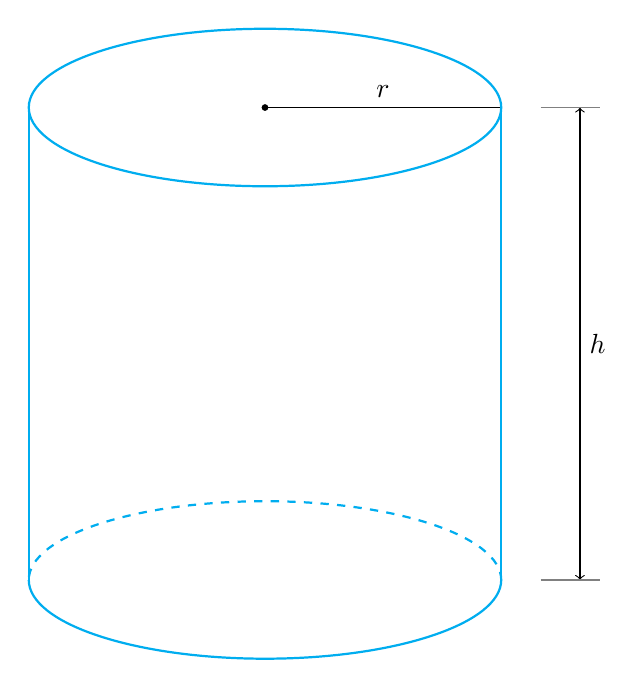
\begin{tikzpicture}
		\def\a{3} % bán trục lớn = bán kính trụ
		\def\b{1} % bán trục nhỏ
		\def\h{6} % chiều cao trụ
		% các chú thích
		\draw (0,\h)--(\a,\h) node[midway, above]{$r$};
		\filldraw (0,\h) circle(1pt); 
		\draw[<->, xshift=1cm] (\a,0)--(\a,\h) node[midway, right] {$h$};
		\draw[gray] (\a,0) ++(0.5cm,0)--+(0.75cm,0) 
		(\a,\h) ++(0.5cm,0)--+(0.75cm,0);
		% vẽ các cạnh bên
		\draw[cyan, thick] (\a,0)--(\a,\h) (-\a,0)--(-\a,\h);
		% vẽ đáy dưới
		\draw[dashed, cyan, thick] (\a,0) arc [x radius=\a, y radius=\b, start angle=0, end angle=180];
		\draw[cyan, thick] (-\a,0) arc [x radius=\a, y radius=\b, start angle=180, end angle=360];
		% vẽ đáy trên
		\draw[cyan, thick]  (0,\h) ellipse (\a cm and \b cm);
	\end{tikzpicture}
\end{document}
%%%%%%%%%%%%%%%%%%%%%%%%%%%%%%%
% Vẽ hình trụ, giả 3D
\documentclass[tikz,border=5mm]{standalone}
\usetikzlibrary{shadings}
\begin{document}
	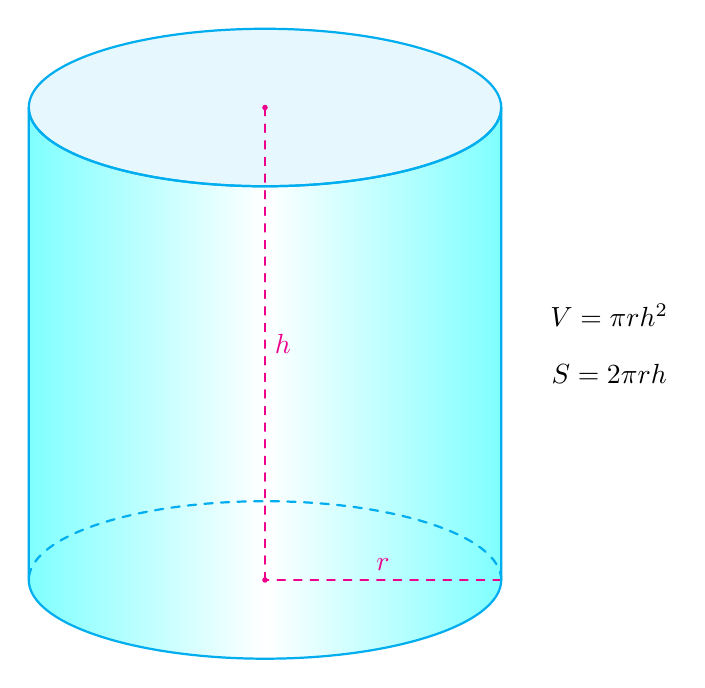
\begin{tikzpicture}[line join=round,line cap=round]
		\def\a{3} % bán trục lớn = bán kính trụ
		\def\b{1} % bán trục nhỏ
		\def\h{6} % chiều cao trụ
		% tạo hiệu ứng 3D: cho màu cyan nhạt (cyan!50)
		% tạo vết nhạt dần từ 2 bên, đến màu trắng ở giữa (thư viện shadings)
		\fill[left color=cyan!50,right color=cyan!50, middle color=white] (\a,0)--
		(\a,\h) arc [x radius=\a, y radius=\b, start angle=0, end angle=-180]--
		(-\a,0) arc [x radius=\a, y radius=\b, start angle=180, end angle=360]--cycle;
		\fill[cyan!10!white]  (0,\h) ellipse (\a cm and \b cm);
		% các chú thích
		\draw[magenta, dashed] (\a,0)--(0,0) node[midway, above]{$r$};
		\draw[magenta, dashed] (0,\h)--(0,0) node[midway, right] {$h$};
		\fill[magenta] (0,0) circle(1pt) (0,\h) circle(1pt); 
		\draw[cyan,thick] (\a,0)--
		(\a,\h) arc [x radius=\a, y radius=\b, start angle=0, end angle=-180]--
		(-\a,\h)--
		(-\a,0) arc [x radius=\a, y radius=\b, start angle=180, end angle=360]--(\a,0)--cycle;
		% vẽ đáy dưới
		\draw[dashed, cyan, thick] (\a,0) arc [x radius=\a, y radius=\b, start angle=0, end angle=180];
		% vẽ đáy trên
		\draw[cyan, thick]  (0,\h) ellipse (\a cm and \b cm);
		\draw (\a,\h/2) node[right=.5cm, align=center] {$V=\pi rh^2$\\[.3cm]$S=2\pi rh$};
	\end{tikzpicture}
\end{document}